\documentclass[a4j,10pt,dvipdfmx]{jarticle}
\usepackage{url}
\usepackage[version=3]{mhchem}
\usepackage{siunitx}
\usepackage[dvipdfmx]{graphicx}
\usepackage{pdfpages}
\title{計算科学} 
\author{学籍番号2120029, 氏名 政野玄空,使ったPC:ChemLab-12}
\date{2021年12月24日}
\begin{document}
\maketitle
\section{10分間テスト}
  1.分子振動による赤外吸収スペクトルの計算と,振動の方向や分子構造と双極子モーメントの関連性を考察する.


  2.双極子モーメントとは共有結合している2つの原子が異なる電気陰性度を持つときに,電気陰性度の高い方から低い方へと発生するエネルギーの総和.
  \section{実験の目的}
  コンピューターの発展に伴い,量子化学を中心とした計算科学が普及している.今回の実験ではコンピューターの計算を通して分子構造の性質を学ぶとともに計算科学の一端にふれることを目的とする.
  \section{実験の原理}
  \subsection{双極子モーメント}
  双極子モーメントとは共有結合している原子の電気陰性度の違いにより,電荷の偏りがある場合に発生するベクトルを持つエネルギーである.
  電荷の値が$+q$,$-q$,重心間の距離が$L$mであるときに双極子モーメント$\mu$は(\ref{mu})で表される.
  \begin{eqnarray}
    \label{mu}
    \mu = qL
  \end{eqnarray}
  電荷の単位はCである.
  双極子モーメントの発生しない分子は無極性分子と呼ばれる.双極子モーメントは分子構造に作用される.
  \subsection{赤外吸収スペクトル}
  分子は絶えず伸縮振動や変角振動をしており,その振動エネルギーは赤外線エネルギーと同等の領域になる.これを振動スペクトルと呼ぶ.
  分子に振動エネルギーと同等の赤外線エネルギーを照射すると,分子による赤外線の吸収が起こる.
  これを赤外吸収スペクトルと呼ぶ.
  二酸化炭素等の温室効果ガスが地表から放出される赤外線エネルギーを吸収して熱を閉じ込めてしまうことが地球温暖化の原因となっている.
  \section{実験手順}
  実験ではSpartranという分子軌道計算ソフトウェアを利用した.
  \subsection{2原子分子の極性と双極子モーメント}
  $\ce{HF}$,$\ce{HCl}$,$\ce{HBr}$の結合距離,双極子モーメント,形式電荷を計算した.形式電荷は(\ref{mu})より算出した.
  \subsection{\ce{CO2}の赤外吸収スペクトル}
  まず\ce{CO2}の赤外吸収スペクトル,平衡構造を計算した.計算した値に0.89をかけて補正し,実測値との誤差を求めた.
  \ce{CO2}の双極子モーメントを計算した.
  \subsection{\ce{CO2}の分子振動と双極子モーメントの変化}
  \ce{CO2}の三種の分子振動と双極子モーメントの変化と結合距離\ce{C = O},結合角\angle\ce{O - C - O}を計算した.
  \subsection{他の温室効果ガスの赤外吸収スペクトル}
  \ce{CHF3}の赤外吸収を計算し,吸収波数と補正値を求めた.分子振動を観察し,伸縮振動か変格振動のいずれかか判断した.
  \section{結果}
  実習1に2原子分子の極性と双極子モーメント,実習2に\ce{CO2}の赤外吸収スペクトル,実習3に\ce{CO2}の分子振動と双極子モーメントの変化,実習5に他の温室効果ガスの赤外吸収スペクトルの結果をまとめた.
  \begin{center}
    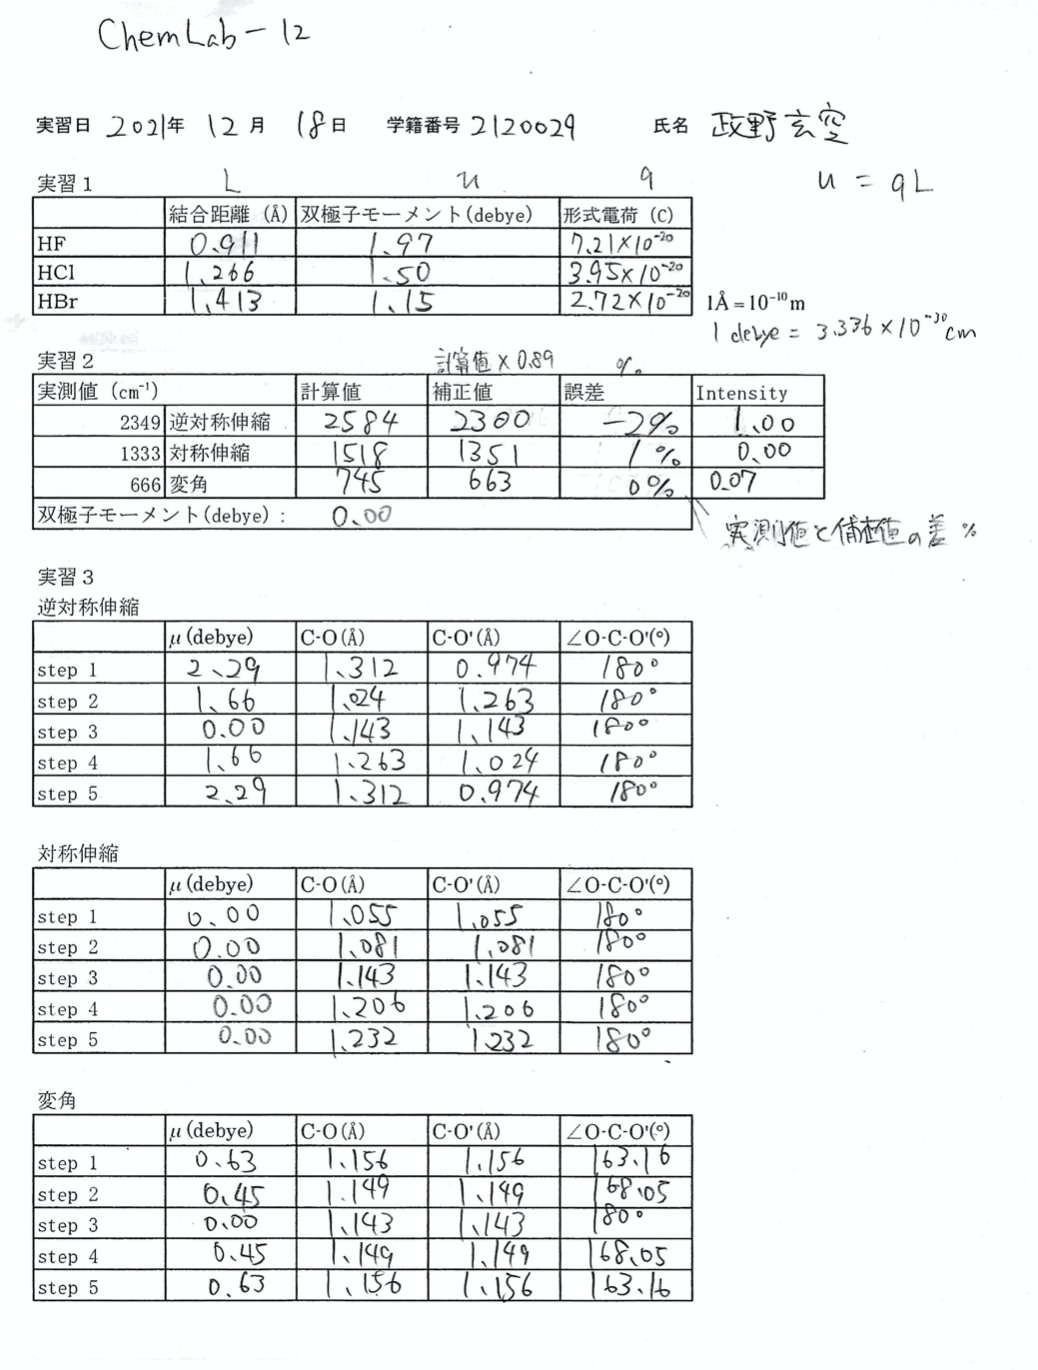
\includegraphics[width=15cm]{hyou1.png}
  \end{center}
  \begin{center}
    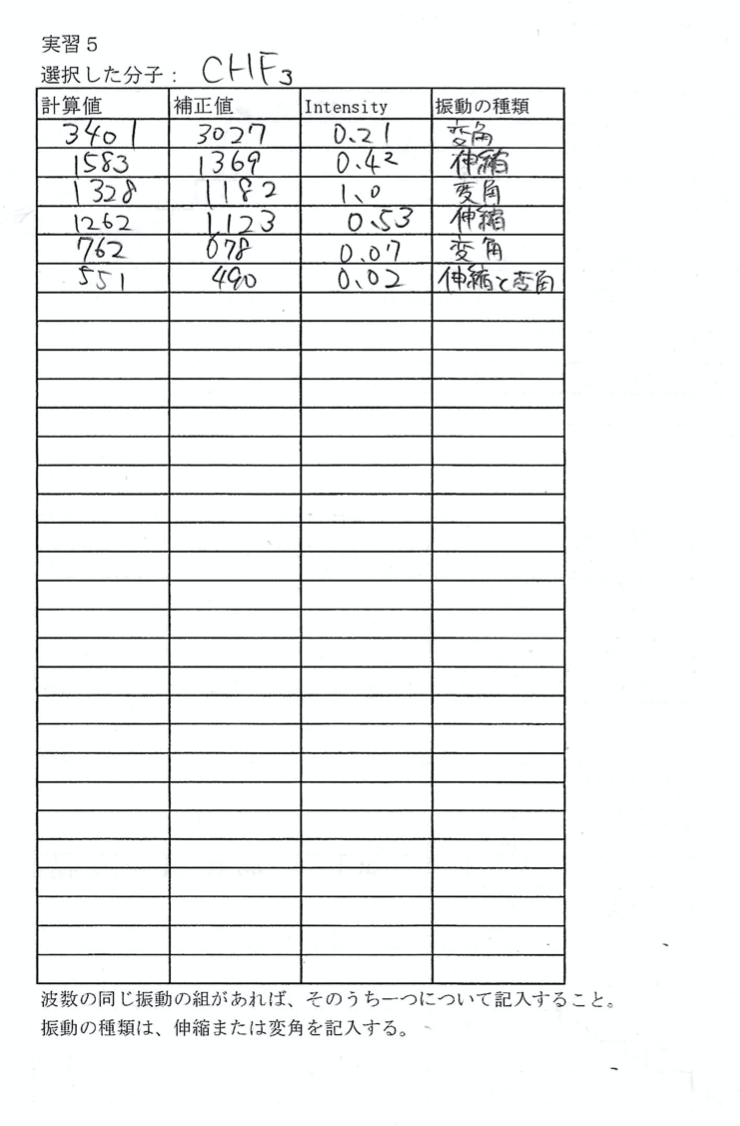
\includegraphics[width=15cm]{hyou2.png}
  \end{center}
  \section{考察}
  実習1の結果と\cite{a}p52より各原子の電気陰性度,H:2.1,F4.0,Cl:3.0,Br:2.8から形式電荷は,電気陰性度の差が大きいほど値も大きくなると考えられる.

  実習2と\cite{a}p50の赤外スペクトルの図より,\ce{CO2}の変格振動は双極子モーメントが変化しており,赤外活性と見ることができ,660$cm^{-1}$付近の赤外線放射量の減衰に対応していると考えられる.一方\ce{CO2}の対象伸縮振動は双極子モーメントの変化がなく赤外不活性なので赤外線を吸収しない.
  また表には書かれていないが,2300$cm^{-1}$あたりも赤外線放射量の減衰が起こっていると考えられ,\ce{CO2}の逆対象伸縮振動は双極子モーメントが変化しており,赤外活性と見ることができ,同様に対応していると見れる.

  実習3より\ce{CO2}の平衡構造の双極子モーメントは最も小さい値の0である.
  \ce{H2},\ce{O2}は同等の原子同士の結合なので双極子モーメントの変化は起こり得ず,赤外不活性と言える.よって赤外線を吸収しない.\ce{H2O}は折れ曲り型の角度のある原子構造になっており,\ce{CO2}と違ってどの振動でも赤外活性となるのではないかと考えられる.よって赤外線を吸収すると考えられる.

  別途資料の演習4より与えられた値を見ても同様の結果になった.また結果からどれも振動数が大きく,\cite{a}p50の赤外スペクトルの図から考察するに\ce{H2O}は\ce{CO2}より赤外線吸収量が少ないと考えられる.

  以下に演習4を添付する.
  また(a),(b),(c)の答えは表上に,(d)はすべて赤外不性,(e)はそれぞれ赤外不活性となる.

  \begin{center}
    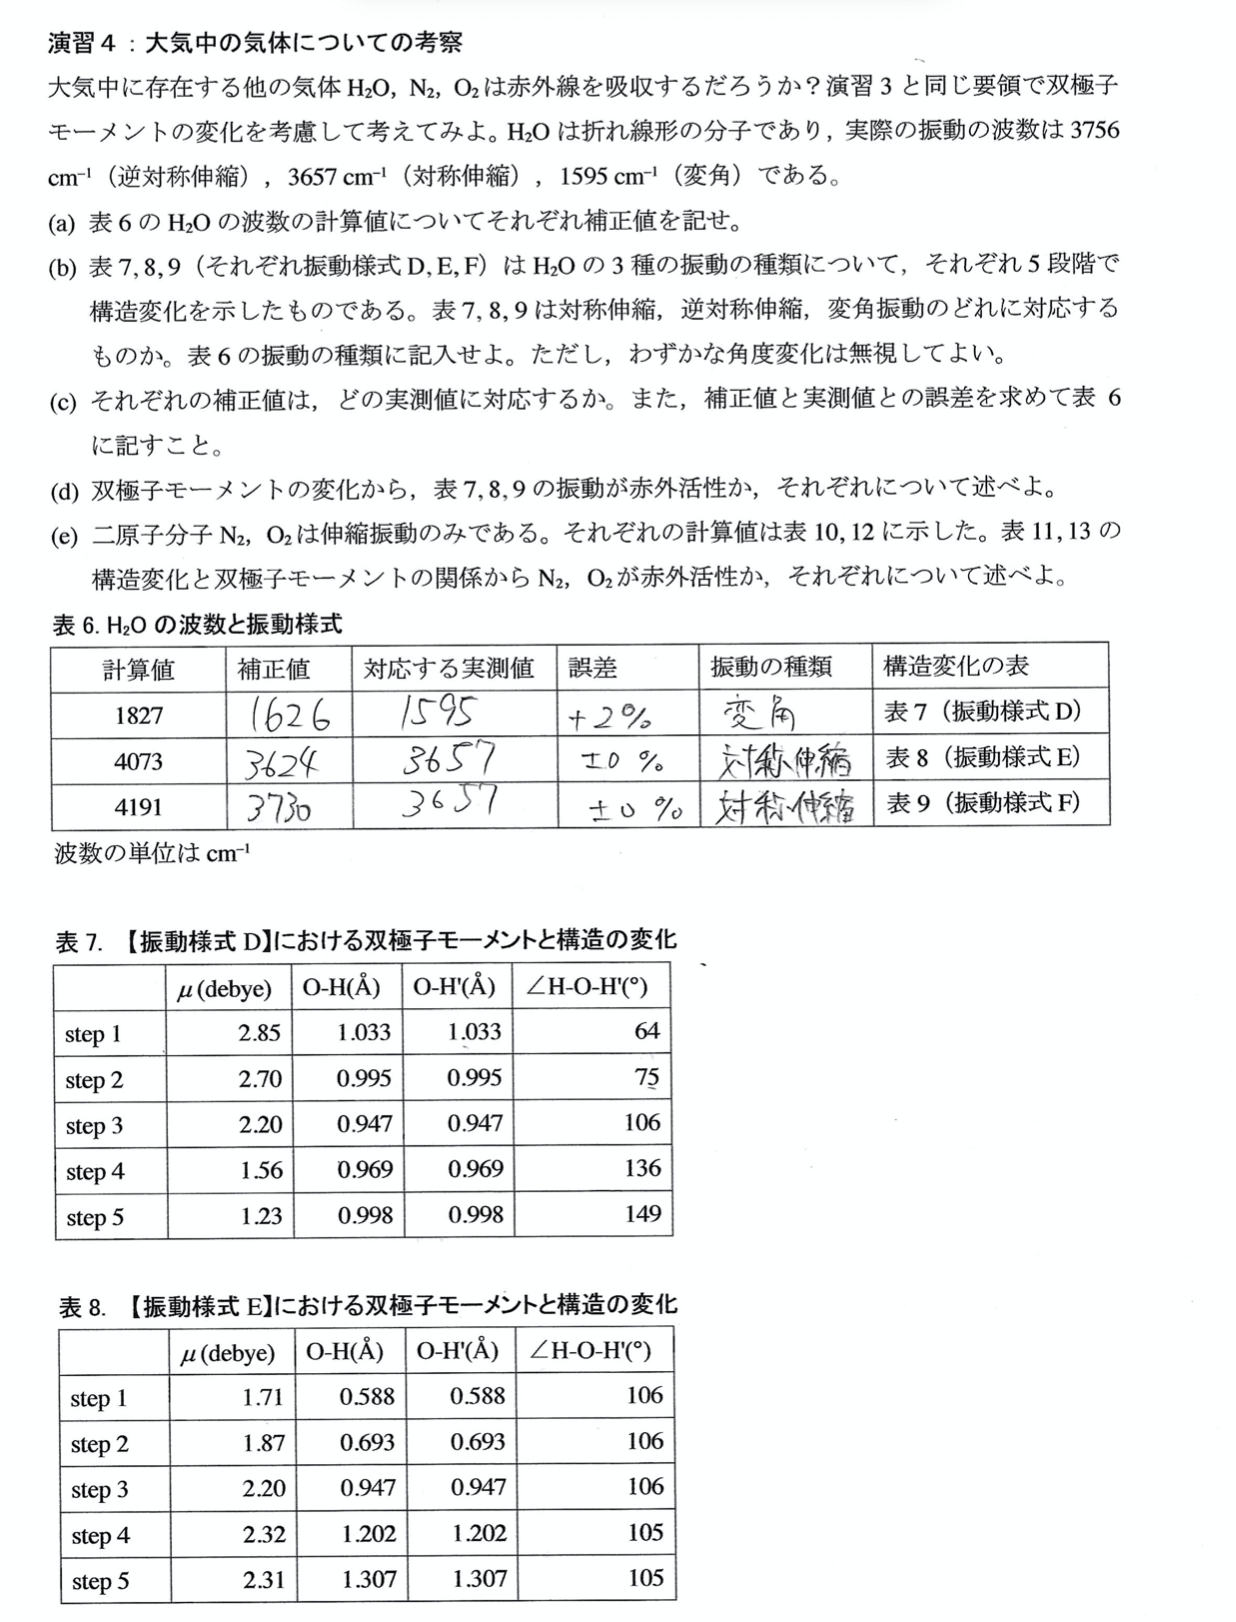
\includegraphics[width=15cm]{en4.png}
  \end{center}
  \begin{center}
    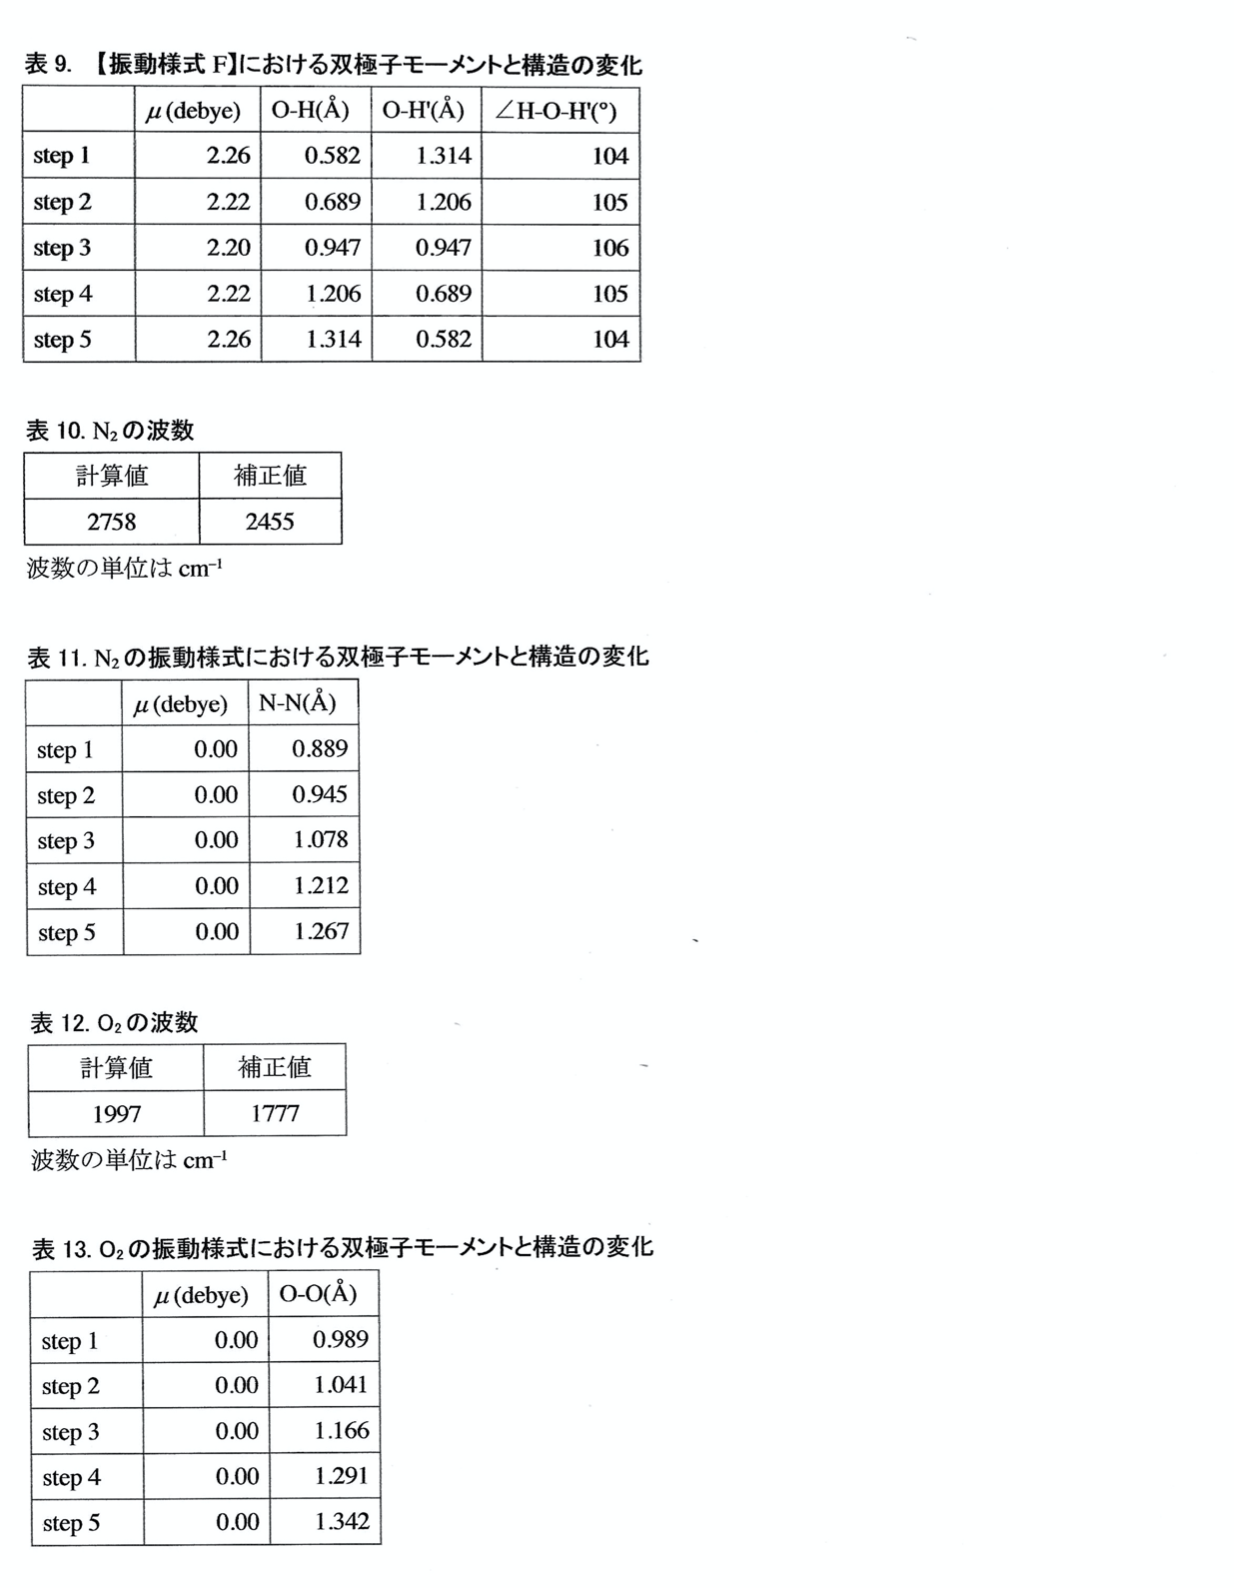
\includegraphics[width=15cm]{en4-1.png}
  \end{center}

  演習5より,今回計算した,\ce{CHF3}はIntencityの値よりどの振動も赤外活性である.
  温室効果ガスとして一番大きな影響を与えそうな振動は\cite{a}p50の赤外スペクトルの図より,計算値が762となった変格振動だと思われる.
  \begin{thebibliography}{9}
    \bibitem{a} 電気通信大学『基礎科学実験』2021年,p50$\sim$55
  \end{thebibliography}
\end{document}
